% !TEX root =  CurvedFoldedDogs.tex

\section{Setup} \label{sec:setup}
\subsection{Definitions}
Throughout the paper, we use the following definition for a curved folded surface:
\begin{definition} \label{def:curved_folded_surface}
A surface $S$ is called a curved folded surface if it is locally isometric to the plane and can be written as a finite union $S = \bigcup S_i $ where each $S_i$ is a $C^2$ developable surfaces termed a \emph{patch}, and the intersections of the patches $S_i \cap S_j$ are either empty or are $C^2$ curves.
\end{definition}
% consists piecewise $C^2$ developable surface whose discontinuities are focused along $C^2$ curves. More formally, 
This definition is suitable for various topologies, such as a cylinder, but throughout this paper we work with surfaces that are isometric to a subset of $\R^2$. Borrowing terms from \cite{origami_book,non_pleated}, we often refer to the surface \emph{crease pattern} as the planar domain $P$ isometric to $S$, subdivided into patches $P_i$ (flattened $S_i$), whose intersection curves are the flattened creases (see \figref{fig:crease_pattern}). Flattened creases with nonzero curvature are said to be curved, while those with vanishing curvature are straight. A crease might be partly curved and partly straight, or curved almost everywhere but with inflection points where the curvature vanishes. When we discuss curved folds, we always assume nonzero curvature, unless specified otherwise \OSH{so, we assume NO inflection points for curved folds?}. The flattened domain boundaries together with the flattened crease curves form a planar arrangement \cite{arrangements}, inducing a planar graph that decomposes $P$ into the planar faces $P_i$. The vertices of this graph are the intersection points of the curves with each other or the boundary curves, which we call \emph{crease vertices}. The \emph{edges} of this graph are the pairwise intersections of the various patches, and we refer to the inner points of these curves as \emph{crease points}, i.e., the points on these curves that are not \emph{crease vertices}. We say that $S$ is \emph{folded} at a crease point $p$ if at that point the patches $S_i,S_j$ sharing it have a tangential discontinuity (see \figref{fig:folded_and_not_folded}).

\begin{figure} [h]
	\centering
	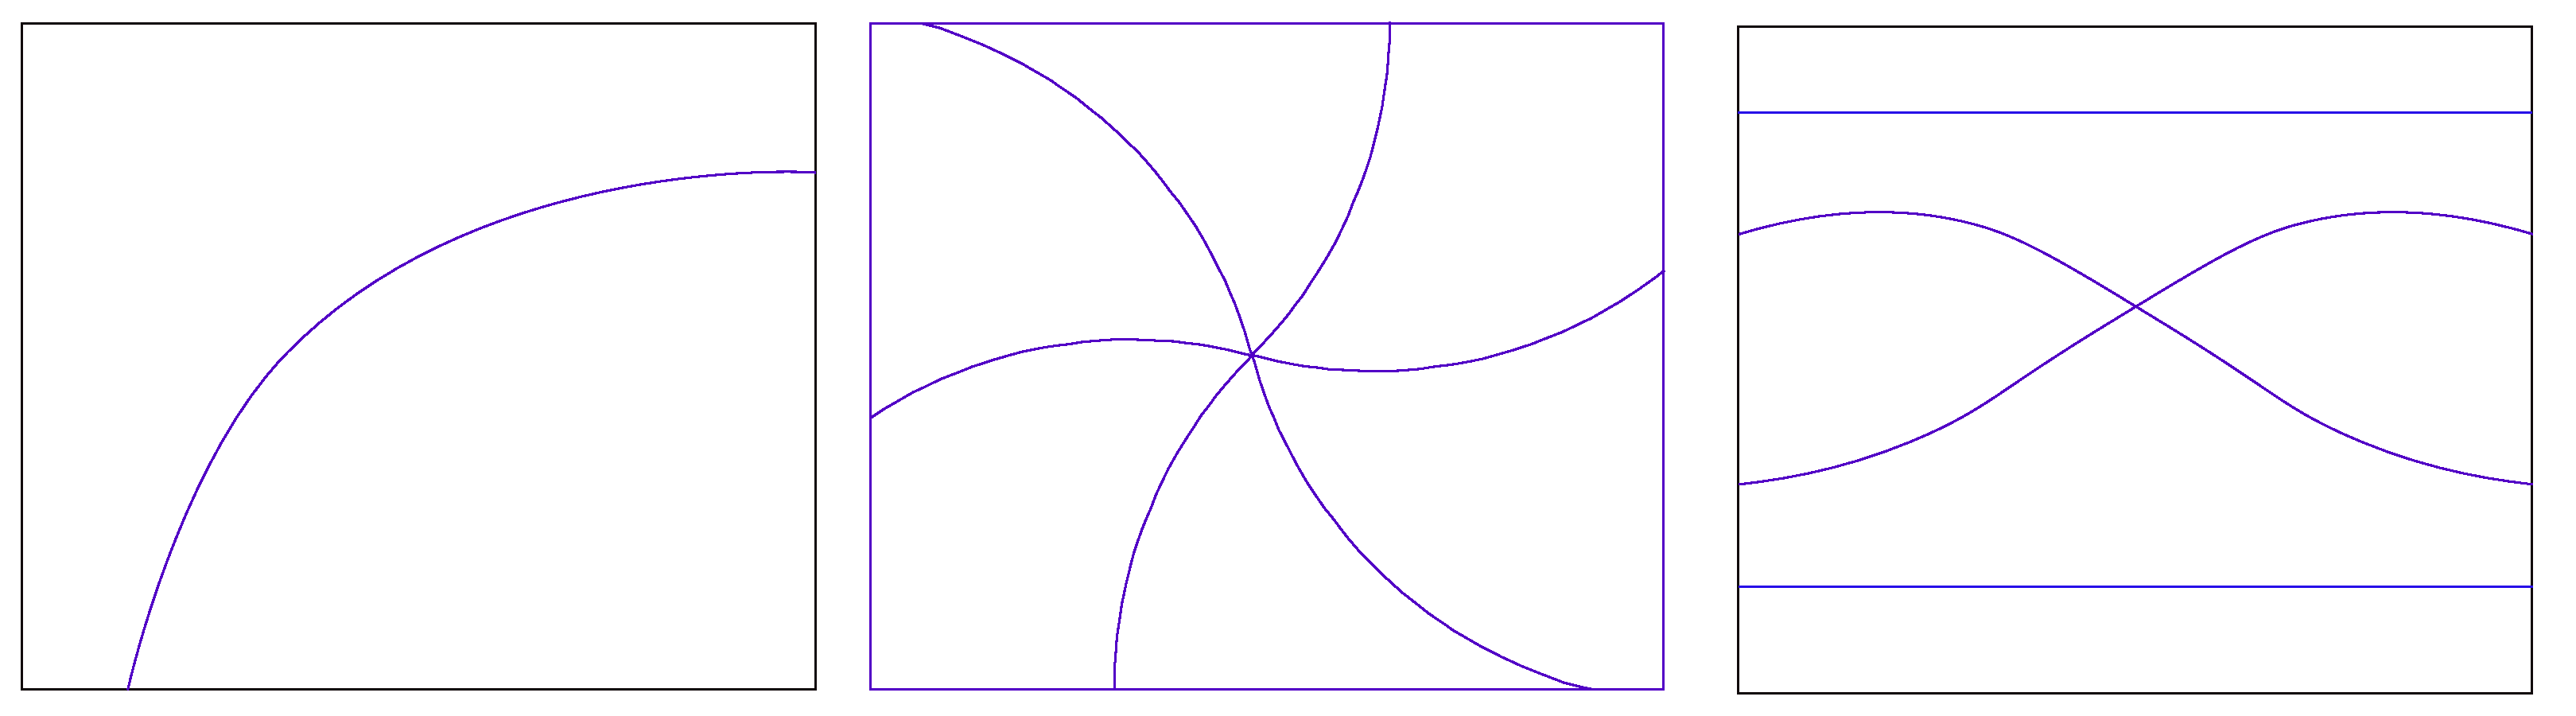
\includegraphics[width=\linewidth]{figures/crease_patterns}
	\caption{Curved crease patterns, decomposing a pattern into multiple components $P_i$ and intersecting at crease vertices. Boundary curves in black, crease curves in blue.}
	\label{fig:crease_pattern}
\end{figure}

We are interested in deformations of curved folded surfaces that keep them curved folded. Viewed separately on each patch $P_i$, these deformations are $C^2$, though they often introduce folds along the creases as tangent plane discontinuities of neighbouring patches. In particular, we are interested in continuous deformations, or deformation flows \cite{rabi2018shape}, which we refer to as curved folding flows. We denote these flows by a continuous map $S(t), 0 \leq t \leq 1$, where each $S(t)$ is a curved folded surface and the flow is $C^2$ when limited to each patch. We often look at the case where the starting point $S(0)$ planar. We apply our tools to model isometric curved flows, which we also refer to as \emph{folding}. These flows can be used to model physical paper or sheet metal folding, though most of our observations and tools can also be used to model curved folding flows that stretch a developable surface while keeping it developable. Non-isometric developable deformations can be useful for design tasks where the a priori flattened shape is unknown \cite{rabi18,rabi2018shape,pottmann_new}.

\subsection{Model} \label{sec:model}
We follow the work of \cite{rabi2018shape} by modeling each patch $P_j$ as a discrete orthogonal geodesic net, together with alignment constraints on their boundaries. Our input is an arrangement of curves representing our crease pattern. On top of this arrangment we place an orthogonal grid while ensuring that every vertex of the arrangement lies on a grid line. We then split the grid into overlapping patches, overlapping along the faces where curves pass. Finally we compute the intersections of the curves with the grid edges and represent the resulting curve points as linear combinations, one for each patch sharing that curve point (see \figref{fig:dogs_from_creases}). Following \cite{rabi18} we maintain continuity across curve points along edges while penalizing deviation of the edge lengths across duplicated quads. 
%\MiR{We just do isometry, but this is not constraint.. is writing this way ok?}

%Given a crease pattern, we create a separate DOG for each segment (see the different colors) and use the boundary constraints as in \cite{rabi2018shape}.
\begin{figure} [h]
	\centering
	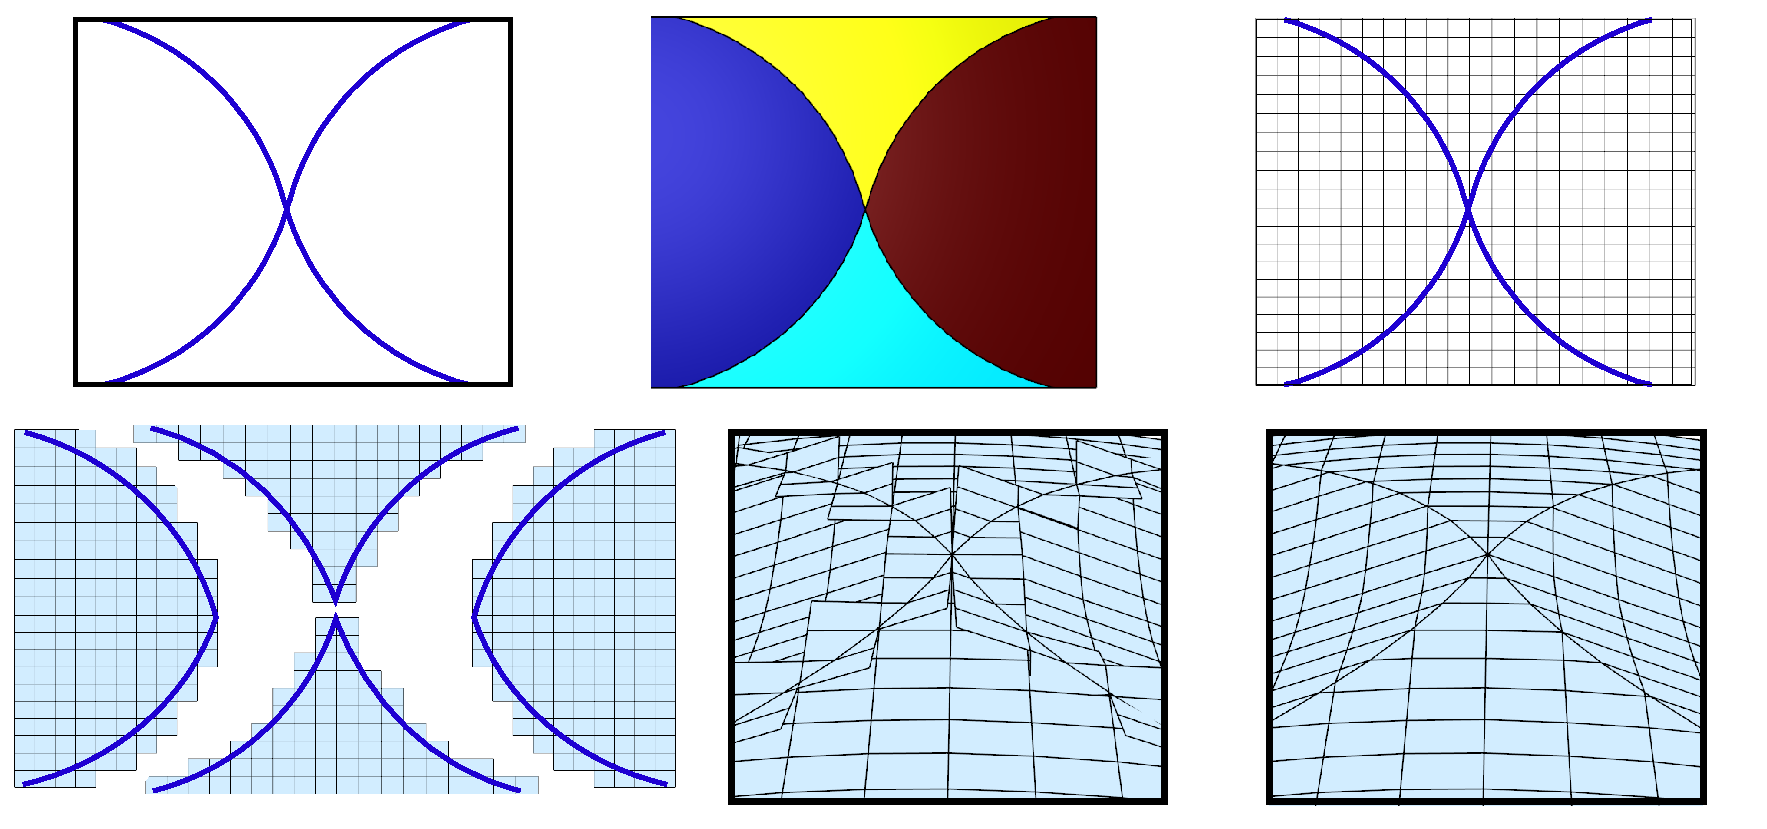
\includegraphics[width=0.8\linewidth]{figures/dogs_from_creases}
	\caption{Representation of a curved folded surfaces, as done in \cite{rabi18}. Up left: An given curves arrangement, representing the domain via its boundary (black), and two curves intersecting along their inflection point at the center of the domain. Up center: The curves segment the domain into $4$ patches, each intersecting two other patches along a partial part of the crease curve. Up right: Placing an orthogonal grid on top of the crease pattern. Down left: We model the surface by having a seperate DOG for each patch, where faces intersecting curves are duplicated along different patches, and the various DOG patches satisfy the continuity constraints specified at \cite{rabi18}. Down center: A deformation of the planar model. Down right: Rendering of the mesh after culling.}
	\label{fig:dogs_from_creases}
	
	
	%representing the domain boundary (black) and creases(blue). In this example the input contain two curves intersecting along their inflection point at the center of the crease pattern. Our input is an arrangement of curves representing the domain boundary (black) and creases (blue). 
\end{figure}

\subsection{Desiderata}
Our goal is to develop tools for the exploration of curved folded shapes on top of piecewise DOGs by means of deformations. Our choices are guided by the two following ground rules for deforming DOGs:
(1) Perform homotopy based optimization, and 
(2) Minimally constraining the DOGs.

%\begin{enumerate}
%  \item Perform homotopy based optimization \label{homotopy_opt}
%  \item Minimally constrain DOGs \label{minimal_const}
%  \item Use accurate functionals \label{accurate_func}
%  \item Use simple functionals
%\end{enumerate}
\emph{Homotopy based optimization} is motivated both theoretically and empirically: Modeling DOGs requires solving highly constrained and nonlinear optimization problems, yet the theory of DOGs guarantees the existence of nearby solutions if one starts at a feasible point. In fact, generally the shape space of DOGs is a smooth manifold \cite{rabi2018shape}. This observation is useful in practice: DOGs exploration has been demonstrated to perform well using smooth flows or homotopy based optimization methods both for handle based deformation tasks as well for more complicated deformations such as curve-constraining flows \cite{rabi2018shape} (see \figref{fig:homotopy_curve}).
\begin{figure} [h]
	\centering
	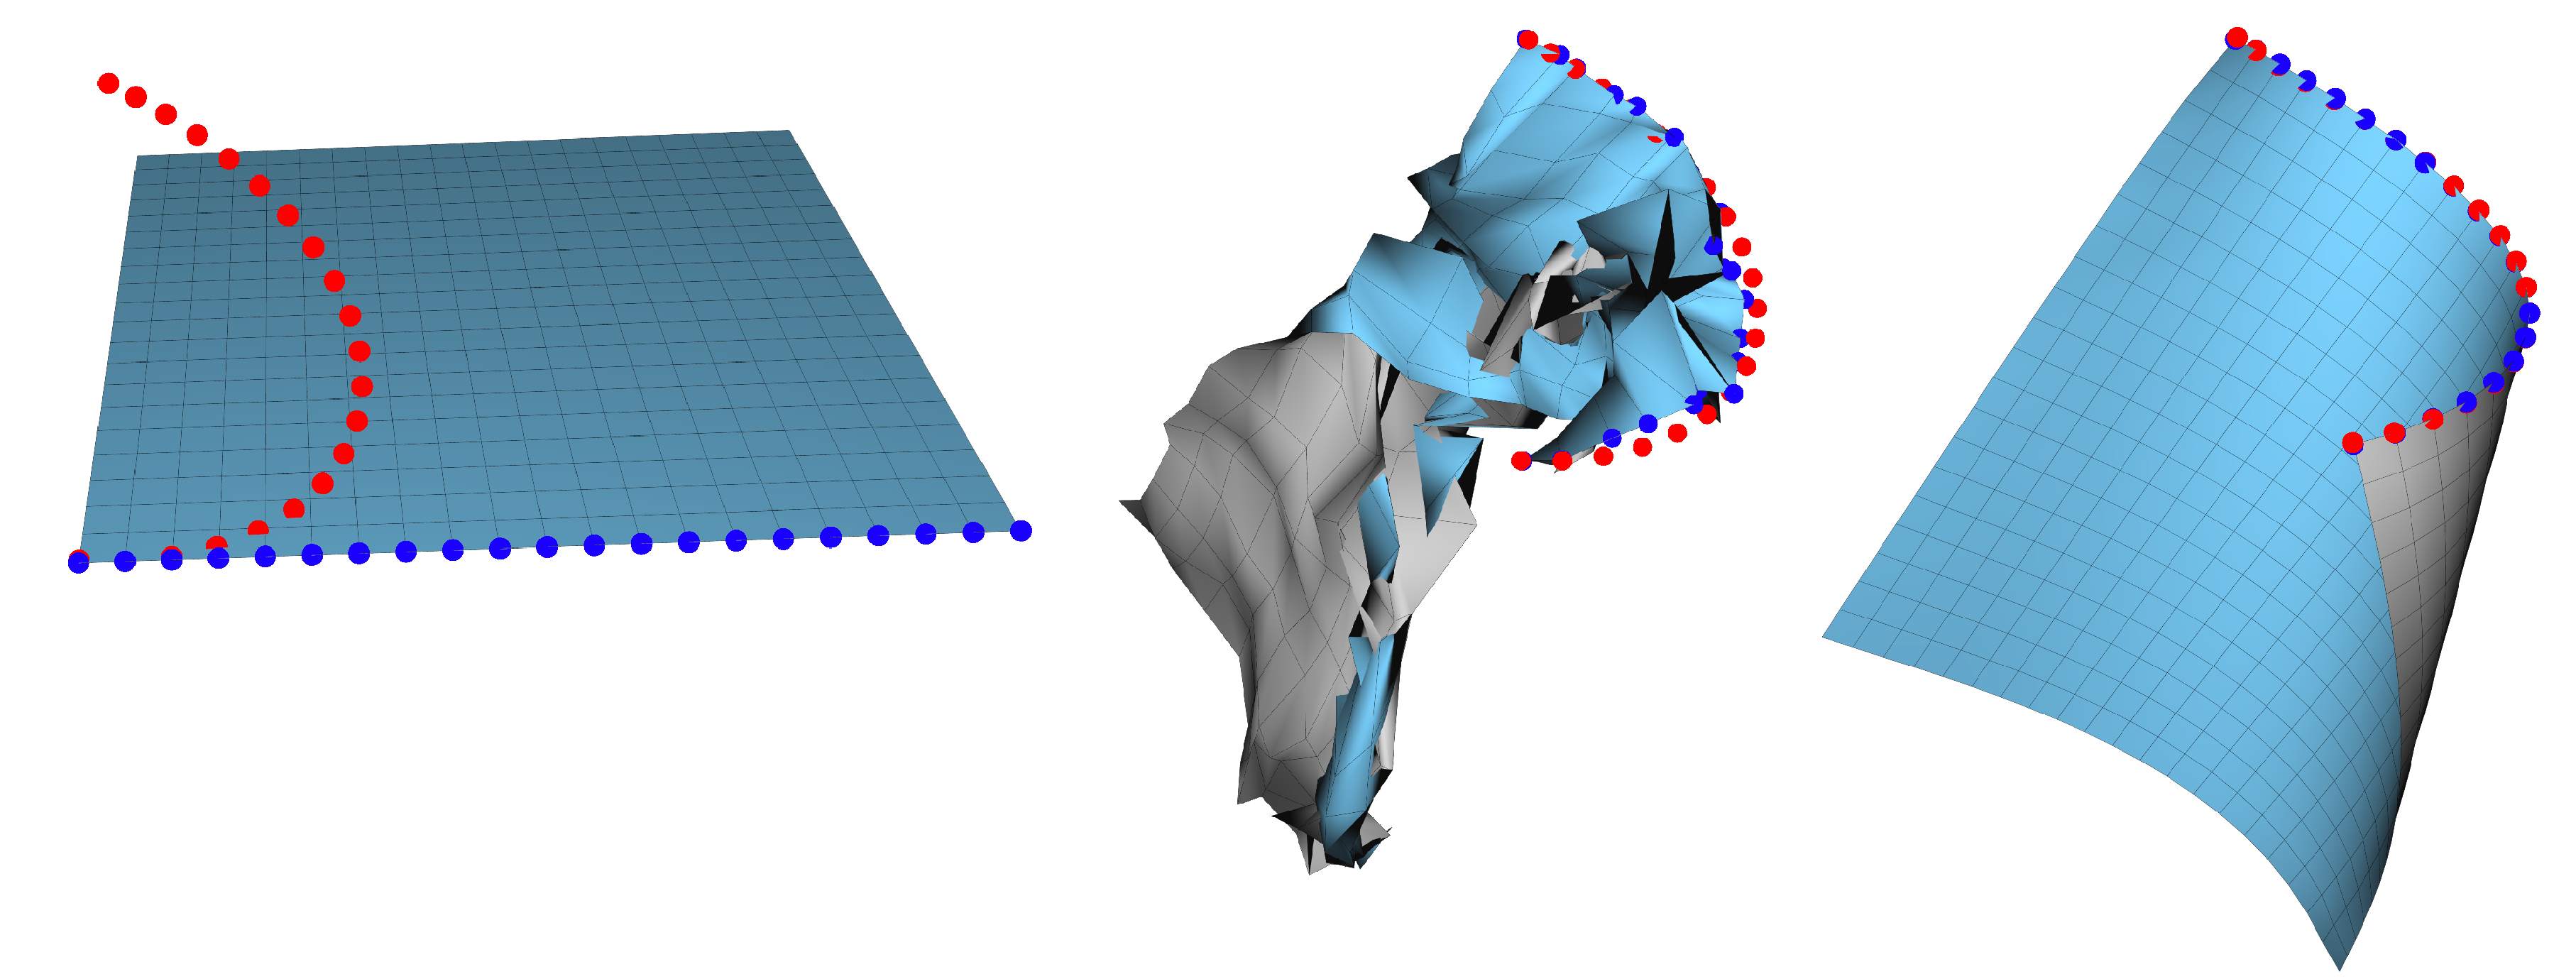
\includegraphics[width=0.9\linewidth]{figures/homotopy_curve.png}
	\caption{Setting soft positional constraints on a curve (left). The same optimization algorithm fails completely when setting all constraints at once, returning a mesh that does not satisfy the non-linear DOG constraints (center). In contrast, using a \emph{curve-constraining flow} \cite{rabi2018shape} returns a smooth DOG (right). The latter approach is a homotopy based method that interpolates the positional constraints.} 
	\label{fig:homotopy_curve}
\end{figure}

\emph{Minimally constraining the DOGs.} Since DOGs are already heavily constrained objects, one needs to carefully choose which quantities to fix by hard constraints, and which ones should be optimized using soft constraints. This is essential in order to avoid locking or ill-posed problems in case the constraint gradients are linearly independent \cite{rabi2018shape}. In particular, the rigidity analysis in \cite{rabi18} demonstrates that one cannot fix all edge lengths, or likewise demand a DOG to also be a Chebyshev net. We note however that this can be done approximately and to a low tolerance, because a DOG is a Chebyshev in the smooth limit, and at the smooth limit there is a rich set of exact isometries. The folding constraints in \secref{sec:folding} are chosen such that they can be satisfied \emph{exactly}. They capture an important characteristic of curved folded surfaces: a folded crease point remains folded under small deformations.
%\textbf{Accurate functionals.} We look for constraints and objectives that are accurate and as often in the case with DOG objectives, converge under sampling of a smooth orthogonal geodesic net \cite{rabi18,rabi2018shape}. \\
%\textbf{Simple functionals.} We strongly prefer sparser objectives with a lower degree as possible. To that end, we leverage the regularity of the DOG meshing and theory on smooth orthogonal geodesic nets in our derivations. \\